\documentclass[letterpaper, 10 pt, conference]{IEEEconf} %
\author{William Baskin, Nicholas Szczecinski and Roger Quinn}
\title{
  {A Biologically Inspired Controller for Efficient Trajectory Execution with Pneumatic Actuated Joints}\\
}
% \date{Day Month Year}
% \date{\today}

% \usepackage[utf8]{inputenc}
% \usepackage[english]{babel}
% \usepackage{csquotes}
\usepackage{graphicx}
\graphicspath{ {images/} }
% \includegraphics[height=6.75in,angle=270]{HW25}

\usepackage[style=ieee, backend=biber]{biblatex}
\addbibresource{references.bib}

\usepackage[hidelinks]{hyperref}
\usepackage{cleveref}

\usepackage{floatrow}

% https://tex.stackexchange.com/questions/119513/cleveref-and-appendix-packages-appendix-referenced-as-section
% \crefname{appsec}{Appendix}{Appendices}

\newcommand{\myref}[1]{\hyperref[#1]{\Cref{#1}}}

%%% math %%%
\usepackage{amsmath, amssymb, amsthm}
% \DeclareMathOperator*{\argmax}{arg\,max}
% \DeclareMathOperator*{\argmin}{arg\,min}

% %%% Code %%%
% \usepackage{color}
% \usepackage{verbatim}
% \usepackage{listings}
% \definecolor{dkgreen}{rgb}{0,0.6,0}
% \definecolor{gray}{rgb}{0.5,0.5,0.5}
% \definecolor{mauve}{rgb}{0.58,0,0.82}

% \lstset{frame=tb,
%   language=Matlab,
%   aboveskip=3mm,
%   belowskip=3mm,
%   showstringspaces=false,
%   columns=flexible,
%   basicstyle={\small\ttfamily},
%   numbers=none,
%   numberstyle=\tiny\color{gray},
%   keywordstyle=\color{blue},
%   commentstyle=\color{dkgreen},
%   stringstyle=\color{mauve},
%   breaklines=true,
%   breakatwhitespace=true,
%   tabsize=3
% }


%%% Packages for the future %%%
% \usepackage{parskip}
% \usepackage{textcomp}
% \usepackage{soul}

\newcommand{\subsubsubsection}{\paragraph}
\newcommand{\bbs}[1]{\section{#1}}
\newcommand{\bbss}[1]{\subsection{#1}}
\newcommand{\bbsss}[1]{\subsubsection{#1}}
\newcommand{\bbssss}[1]{\subsubsubsection{#1}}

\newcommand{\norm}[1]{\left\lVert#1\right\rVert}

\begin{document}
\maketitle

\begin{abstract}
\label{chap:abstract}
This research develops a new synthetic nervous system for control of joints using pneumatic actuators in order to create a more efficient and adaptable walking robot system. This design implements new features not previously seen in a control oriented nervous system. It develops 3 major design components not previously used for control of antagonistic pneumatic actuators. It uses an internal model of the actuators to estimate the state of the joint. It uses internal estimates of the dynamics of the joint to continually optimize the control output. Additionally, it updates its own internal system model with a memory-like loop to allow the controller to adapt to any joint and trajectory. The controller allows for the replacement of proportional or other control designs with a learning system that decreases wasted antagonistic muscle activation and wasted energy, decreases phase lag and increases trajectory tracking accuracy.
\end{abstract}

\bbs{Introduction} % and Lit Review
\label{chap:introduction}

Walking robots offer many advantages over wheeled robots or other types
of locomotion. Wheeled or tracked vehicles are unable to access over half
of the earth's landmass. \cite{BigDog} Further, many areas in which humans
operate are designed for walking as opposed to rolling, so a successful walking 
robot has increased mobility in environments designed for human walking. On the
other hand, walking robots are harder to control than their wheeled 
counterparts.

Many robots have looked to biological inspiration to increase the mobility and
ease of control of robots. In particular, many biological systems have increased
redundancy to aid in balance with many animals, including dogs and cats, walking
on 4 or more legs. The inspiration taken varies from imitating gait timing to
help coordinate simple legs to completely mimicing musculoskeletal layout. The
Puppy robot was designed to mimic the operation of a large canine walking in
the sagittal plane. \cite{PuppyDesign}

Another advantage that animals have over most robots is their actuators.
Biological muscles are compliant and are a key part to how animals walk. Many
robots use electric motors or hydraulic actuators to actuate joints, which can
mean that other biologically inspired design decisions aren't necessarily 
optimal. Puppy chose to use pneumatic artificial muscles, which have a higher
power to weight ratio than other designs and offer similar compliance and
behavior to biological muscles. \cite{Tavakoli2008} Typically seen as a 
limitation, pneumatic muscles as actuators apply force during contraction, so 
they need to be used in antagonistic pairs. While this increases the complexity
of the robot, it also allows for further bio-inspiration in the robot design
and control system.

One of the major tradeoffs for pneumatic muscles is that they exhibit 
non-linear behavior in both static and dynamic control situations.
\cite{HuntPMuscles, DynamicPMuscles} This has 
motivated the designs of new types of controllers to overcome the non-linear
behavior through adaptation in the controller. In \cite{Jahanabadi2009}, the
authors propose a system called ``Active Force Control" where a neural network
is used to learn non-linear properties of the actuator and controlled mass.
The network is run in an inner control loop and the output of the network is
used to present the control situation in a linearized fashion to an outer PID
control system. The results suggest that a system model of the nonlinear 
properties of the actuators decreases positional error. The work was
applied to controlling a vertical trolley and used a neural network as a black
box for modelling the system, so there is an opportunity for improving the 
system and its application to controlling Puppy's rotational joints. 
In \cite{Wang2013}, a model-based controller was used to control the actuation
of a revolute joint with pneumatic muscles. The author's system allowed for
decreased antagonistic muscle overlap at high accelerations combined with a 
high stiffness, high overlap controller for precise position tracking in near
static situations. This adapting system was shown to be effective in their
results; however, it doesn't account for estimating changing properties of the
robot system that might reduce the effectiveness of the model.

A combination of these two types of controllers offers insight into how to build
an effective joint controller for Puppy. One further area of potential 
improvment over existing designs is the incorporation of biological inspiration
within the controller itself. In \cite{NickFunctionalSubnetwork}, the authors
demonstrate a method for using a dynamic, biologically accurate model of neurons
to develop models of neurons for controlling physical systems. The work in the 
paper describes how to create building blocks such as arithmetic operations,
differentiation or integration. These components can then be used together to 
recursively create new controller architectures that use biological inspiration
taken from literature for controlling legged robots and combine it with an
efficient system for engineering the correct control responses. Together,
existing literature suggests that a neuron-based controller that adapts to the
properties of the muscles and the joints that it controls offers a new
architecture for more efficient and more accurate control of pneumatic muscle-
actuated robots.

In this paper, we show the design process for a new adapting controller. The
design of the controller itself is discussed in \myref{chap:controller_design}.
The implementation of the controller within a synthetic nervous system is 
discussed in \myref{chap:neuron_design}. The results are shown in \myref{chap:results} and discussed in \myref{chap:discussion}.

\bbs{Controller Design}
\label{chap:controller_design}

The controller design has 3 major goals derived from
requirements and challenges faced with a neural implementation in
\cite{HuntPhDThesis}.

\begin{enumerate}
\item Decrease torque errors between neuron desired model and executed torques
\item Minimize phase shift between desired and achieved trajectory
\item Increase position accuracy to less than 5 degrees from maximum desired
position
\end{enumerate}

In order to achieve these 3 goals, 3 areas of improvement were identified:
sensor fusion, an optimizing internal loop and a better system model.

\bbss{Sensor Fusion}

The goal of the sensor fusion system is to provide an accurate measure of the
current state of the joint for the rest of the controller. The joint is defined
by 5 related parameters: position, velocity, acceleration and the pressure in
each of the antagonistic actuators.

While more complex methods are possible, the first controller prototype used
a finite divided difference to estimate the velocity of the joint from the
measured position. The acceleration can be estimated one of two ways: a second
numerical derivative or by using knowledge of how the pressure in the actuators
applies force to the joint itself. The first method was easier to implement in
code. The second method derived a better result when implemented in neurons (see
\myref{chap:neuron_design}).

The internal estimation of the acceleration based on pressure comes from \cite{HuntPMuscles}.

To calculate a pressure from a force and position, the following model is used:

\begin{equation}
P = a_{0} + a_{1} * tan(a_{2} (\dfrac{k}{a_{4} * F + k_{max}} + a_{3})) + a_{5} * F + a_{6} * S
\end{equation}

\begin{equation}
k_{max} = \dfrac{L_{rest} - L_{620 kPa}}{L_{rest}}
\end{equation}

\begin{equation}
k = \dfrac{L_{rest} - L_{angle}}{L_{rest}}
\end{equation}

\begin{equation}
L_{angle} = L_{0} - L_{1} cos(\alpha + \theta)
\end{equation}

\begin{equation}
F = \dfrac{T}{d cos(\beta + \theta)}
\end{equation}

$\alpha, \beta, d, L_{rest}$ and $L_{620 kPa}$ represent the parameters for a 
particular actuator. The $a$ values represent optimized parameters
for the generalized model that adjusts to all actuators. See \cite{HuntPMuscles}
for more details. Once the torque is calculated, the 
estimation of acceleration comes from the internal estimation of the joint's mass, damping and conservative forces.

\bbss{Optimizing Torque Control}

Given the current state of the joint, a binary search algorithm is used to
estimate the optimal control torque. This overcomes limitations with inverting
a complex internal model, but allows for iterative improvement with known bounds
based on the maximum and minimum torque output of the joint at its current 
state.

At each step in the binary search, a forward model is used to evolve the state 
forward at a fixed interval. Originally, this was done with a complete physics
model, but over time the model was simplified down to 3 parameters: inertia, 
damping and conservative load. This simplified internal model was used to 
estimate the ending position of the joint after an application of a given 
torque. The binary search procedure repeatedly shrinks the bounds around the 
optimal torque. Once an optimal torque range is determined, the state and torque
can be used to select the proper pressures for each actuator, with either a 
fixed or varying antagonistic overlap.

Converting from a desired torque to pressure for a single actuator follows
the model expressed above:

\begin{equation}
P = a_{0} + a_{1} * tan(a_{2} (\dfrac{k}{a_{4} * F + k_{max}} + a_{3})) + a_{5} * F + a_{6} * S
\end{equation}

One complicated aspect of implementing conversion from the desired torque to 
pressures in the system is the
knowledge of the underlying control scheme. As described in \cite{HuntPMuscles},
the underlying controller implements a bang-bang algorithm. This means that 
there is some uncontrolled variation in the torque. This means that there is a
range of desired torques that may output the same control. This is modeled as
part of the binary search process, where a window of torques is identified, and
the most likely control torque is selected.

\bbss{System Modeling and Improvement}
\label{sec:systemImprovement}

The original model for updating the weights on the system was to calculate the
intended sign of the error correction for the damping and load estimates and 
then perform a small weight adjustment in that direction. This allows for 
simple, fast calculations and a stable update because there are no large 
changes made. Additionally, there is an easy option for weighting towards 
under- or over-estimating a variable. In general, it is preferable to 
under-estimate a variable such as interia because this lowers the estimated 
torque required, leading to some undershooting of a given value but avoiding
large, underdamped oscillation.

Direct analysis of sources of error suggests a more precise method for updating
the estimated damping and load on the joint. Assuming the three factors characterize the significant dynamics of the joint, the equation for calculating acceleration is as follows:

\begin{equation}
M * \ddot{\theta} + C * \dot{\theta} + N * sin(\theta) = \tau
\end{equation}

This leads to the calculation of acceleration as:

\begin{equation}
\ddot{\theta}_{act} = \dfrac{\tau}{M} - \dfrac{C \dot{\theta}_{0}}{M} - \dfrac{N sin(\theta)}{M}
\end{equation}

Assuming error comes from parameter estimation the error terms can be written as
follows:

\begin{equation}
\ddot{\theta}_{err} = - \dfrac{1}{M}
(C_{err} \dot{\theta}_{0} + N_{err})
\end{equation}

This error in acceleration can be directly measured by comparing the estimated
position and the sensed position at the next control step. After propagating error from acceleration to position, the equation is as follows:

\begin{equation}
\theta_{err} = - \dfrac{\delta t^{2}}{2M}(C_{err} \dot{\theta}_{0} + N_{err} sin(\theta))
\end{equation}

To convert the equation into a form that can be used to update the damping and
load internal estimates:

\begin{equation}
C_{err} = \lambda \dot{\theta}, N_{err} = \dfrac{\lambda}{sin(\theta)}
\end{equation}

where

\begin{equation}
\lambda 
=
- \dfrac{2M}{\delta t^{2} (1 + \dot{\theta}_{0}^{2})} \theta_{err}
\end{equation}

This analysis has a singular point when both $\theta = 0$ and $\dot{\theta} = 0$. In this case, there is no damping effect and no torque applied from a static
load. Therefore, there is no information to quantify their update and the internal update is paused.

\bbs{Neuron Design}
\label{chap:neuron_design}

The neuron controller network is made up of a set of engineered synapses
designed to emulate arithmetic operations. These can be grouped into two
categories: excitatory neurons and inhibitory neurons. Most neurons were tuned
via an optimization process to identify the best equilibrium potential and
synaptic conductance based on equations defined in 
\cite{NickFunctionalSubnetwork}. Some involved some hand tuning for modeling custom behavior.

One key design pattern not seen among other neuron designs is the use of two
neurons to represent a single value centered around 0. In this case, one neuron 
is active when the value is positive and zero otherwise. The second represents 
negative values in the same way. This doubles the precision of the value 
represented by the neurons. Also, it allows for a more accurate representation of a zero value, which is instrumental when comparing two values.

\bbss{Sensor Fusion}

The sensor fusion neuron network performs essentially the same function as the
sensor fusion network in the prototype controller. In this case, 3 neurons
represent the 3 sensor inputs available in a joint: position (``Theta"),
extension muscle pressure (``Ext Pres") and flexion muscle pressure
(``Flx Pres"). The outputs for the network are the estimates for current 
position, velocity and acceleration.

\bbsss{Velocity Estimation}

The velocity network is based on the Differentiator network. 
The one major change from the network,
as presented, is the inclusion of a second $U_{post}$ neuron to 
represent the negative derivative of the position (negative velocity), following the dual-neuron design pattern outlined above.

\bbsss{Acceleration Estimation}
\label{sec:accelerationEstimation}

The acceleration network uses 4 functional sub-network components. The first component is the pressure estimation. This converts a torque estimate internal to the acceleration estimation network into the expected pressure for the extension actuator (with the same network applied to the flexion actuator). This is used within a feedback loop to minimize the error between the input pressures and the torque applied by the muscle. This is an approximation of Newton's method for finding a root, in this case used to match a torque estimate to a pressure input. The torque estimate itself is stored in an integrator pair for use in the rest of the network. The last component is a 3 stage process where damping, static loads and inertial effects are applied to the estimated torque to produce an acceleration estimate.

\bbss{Torque Optimization}

The torque optimization network performs the same function as the torque optmization step in the torque controller; however, it uses Newton's method instead of a bisecting search to estimate the optimal torque.

The torque optimization loop is built around a feedback loop similar to the internal feedback loop in the acceleration estimation discussed in \myref{sec:accelerationEstimation}. In this loop, a torque estimate is passed through a velocity modifier and a position modifier to estimate the change in state for the given torque after being converted to acceleration with damping, load and inertial effects. This is compared to the desired state from a central pattern generator (CPG) and the torque is updated to minimize this error.

Newton's method is not guarunteed to converge; however, in this application with this error function, it will always converge. The derivative of the predicted future position with respect to the initial acceleration estimate is a constant term, so there will only be one root where the feedback loop will terminate.

\begin{equation}
\dfrac{\partial \theta_{future}}{\partial \ddot{\theta}} = \delta t^{2}
\end{equation}

\bbss{System Modeling}

The original implementation of the system update model was a relatively simple approximation of the equation given in \myref{sec:systemImprovement}.

\begin{equation}
C_{err} = \lambda \dot{\theta}, N_{err} = \dfrac{\lambda}{sin(\theta)}
\end{equation}

\begin{equation}
\lambda 
=
- \dfrac{2M}{\delta t^{2} (1 + \dot{\theta}_{0}^{2})} \theta_{err}
\end{equation}

The original assumption was that a gain term can be added that encompases both a translation from an arbitrary range of values to the fixed range available in the neuron (20 mV). This absorbs the $\frac{2}{\delta t^{2}}$ term. This leaves
the mass term and the divison by $1 + \dot{\theta}^{2}$. The mass term is included with a multiplication synapse. 

The key original simplification was that
dividing by $1 + \dot{\theta}^{2}$ is a good approximation for the signal division synapse discussed in \cite{NickFunctionalSubnetwork}. This allowed for
just a single step to calculate $\lambda$.

The additional complexity in the neuron network comes from the need to have the $C_{err}$ term change sign with changes in sign of both the positional error term and the state velocity. This was accomplished with the help of the dual-neuron representation of these values. This design pattern allows for all pairs of edges (positive-positive, positive-negative, negative-positive, negative-negative) to be connected, and then these neurons are connected to the correct sign output neurons. This network only works because only one of each pair of inputs will be active (the other will be at or below its resting potential), so only one of the 4 intermediate neurons will be active, activating one of the two output neurons. This 4 way cross achieves the ability to flip the sign of the output based on velocity and position error sign to correctly calculate $C_{err}$.

\bbs{Results}
\label{chap:results}

\bbss{Sensor Fusion}

The two key estimates made within the sensor fusion sub-network: velocity and
acceleration. Both controllers were tested against sin waves of known
frequencies. See \myref{fig:TestVelPos} and \myref{fig:TestVelNeg}.

% TODO(buckbaskin): bode plot? for positive and negative? in discussion?

\begin{figure*}
\begin{floatrow}
\ffigbox{%
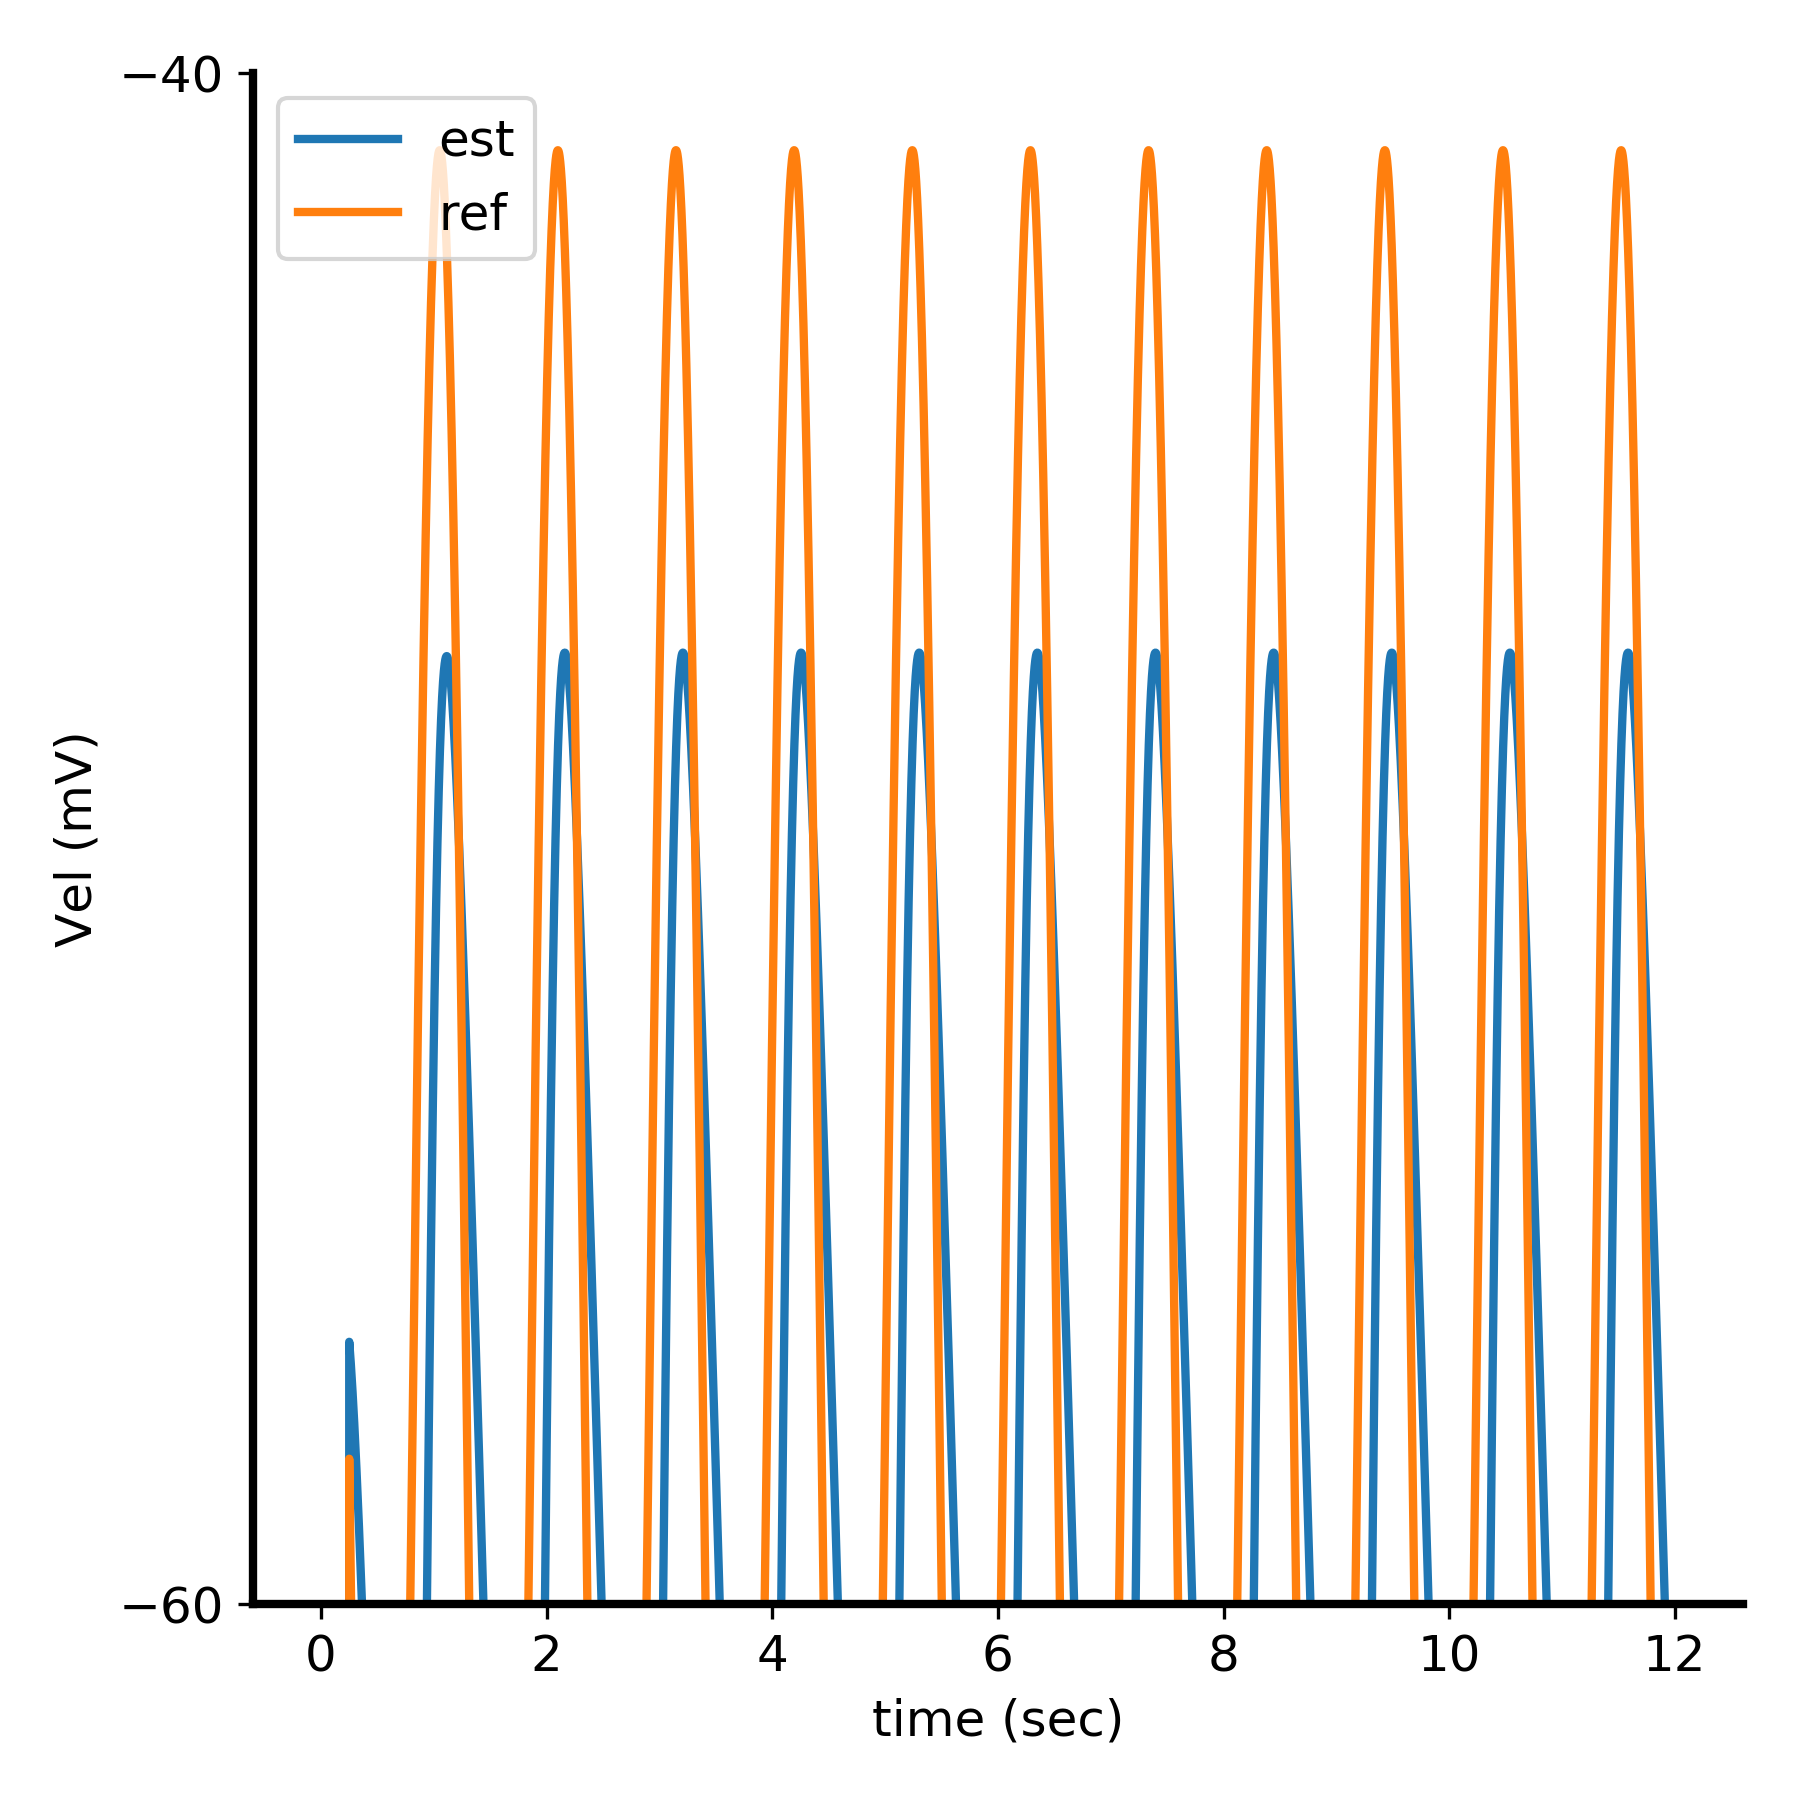
\includegraphics[width=3in]{results/TestVelPos}
}{%
\caption{Positive Velocity Testing (Reference in orange)}
\label{fig:TestVelPos}
}

\ffigbox{%
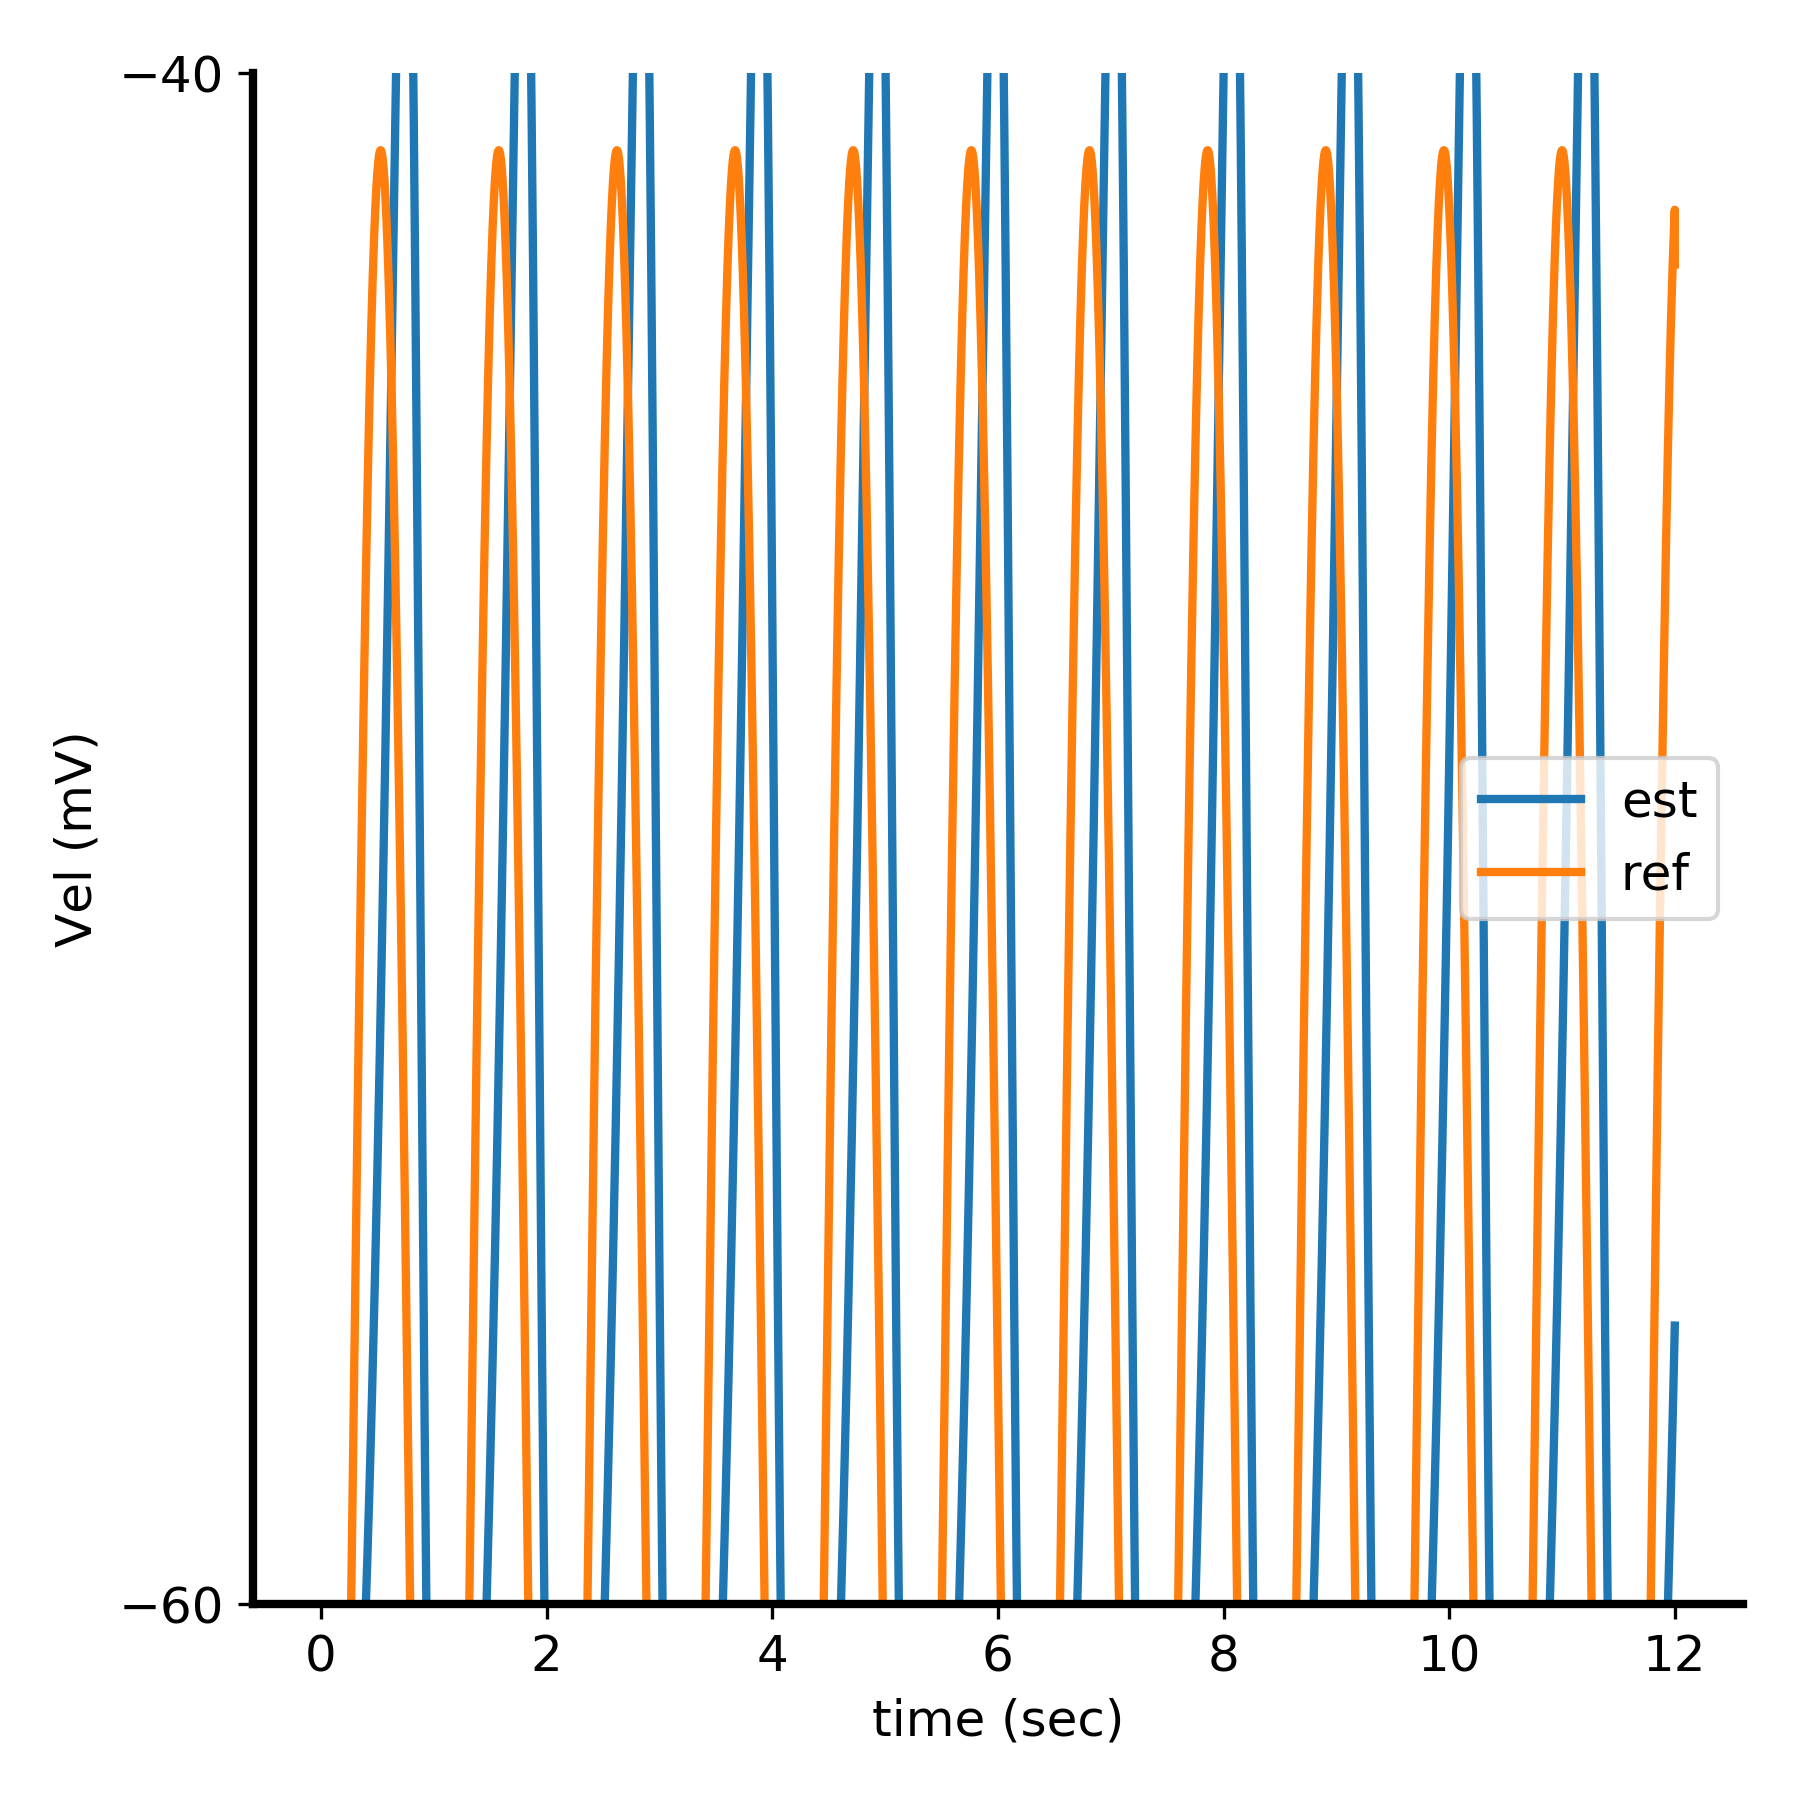
\includegraphics[width=3in]{results/TestVelNeg}
}{%
\caption{Negative Velocity Testing}
\label{fig:TestVelNeg}
}
\end{floatrow}
\begin{floatrow}
\ffigbox{%
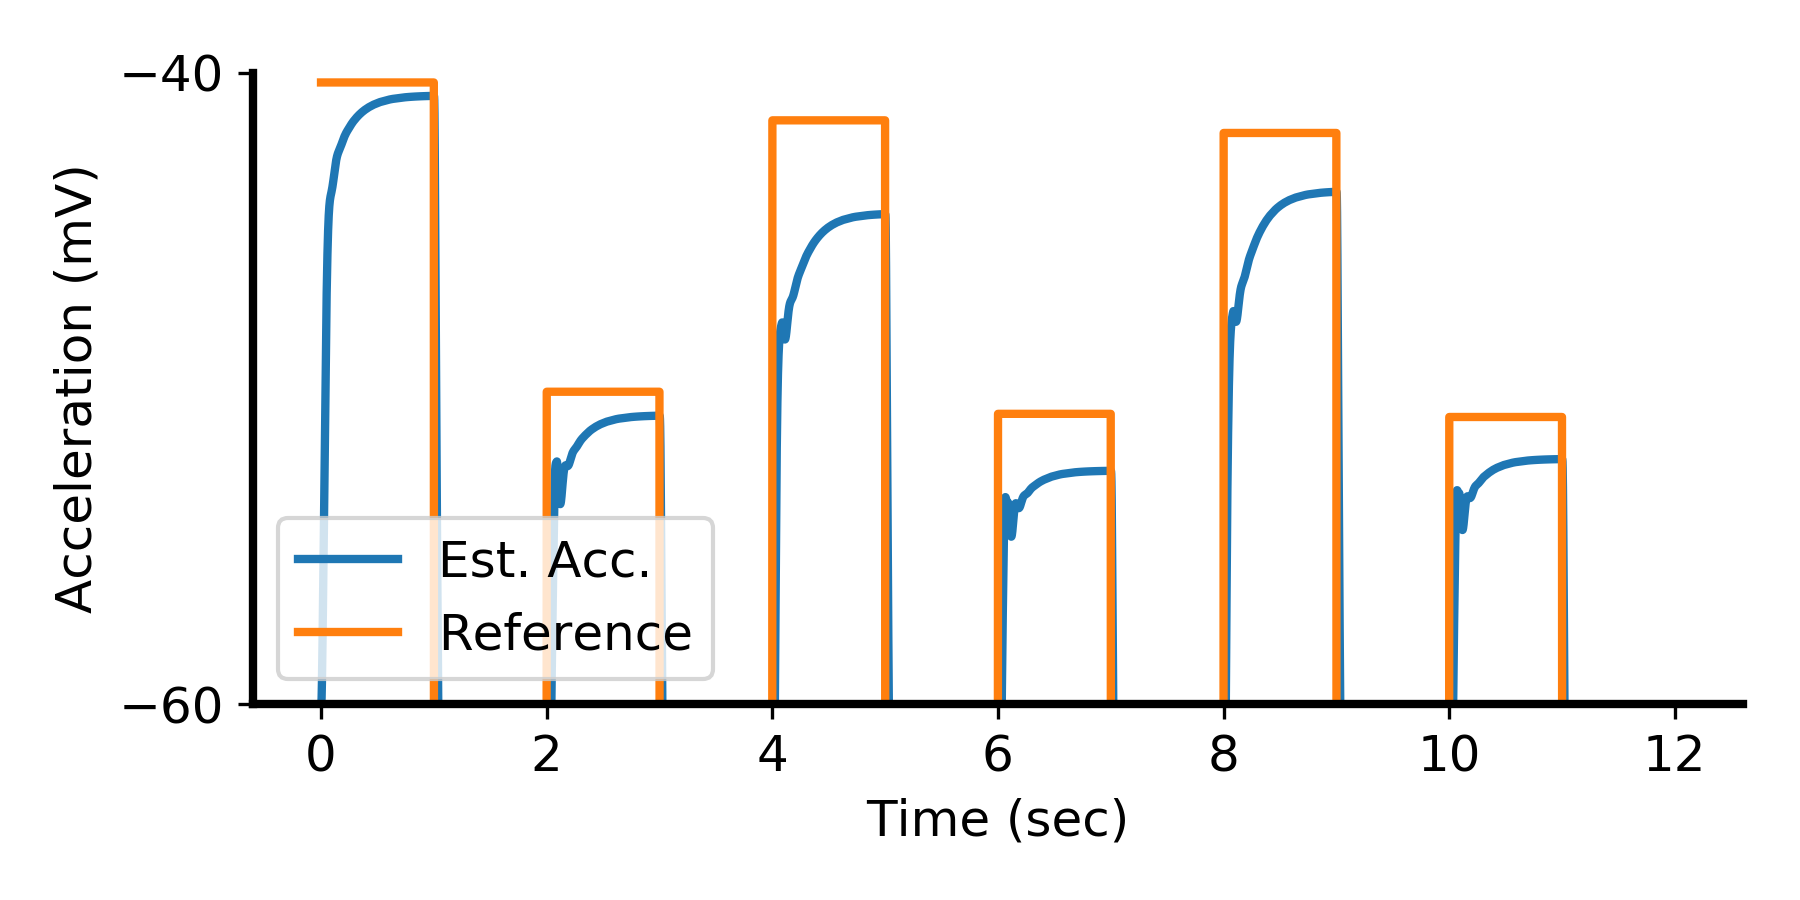
\includegraphics[width=3in]{results/TestAccelPos}
}{%
\caption{Positive Acceleration Testing}
\label{fig:TestAccelPos}
}

\ffigbox{%
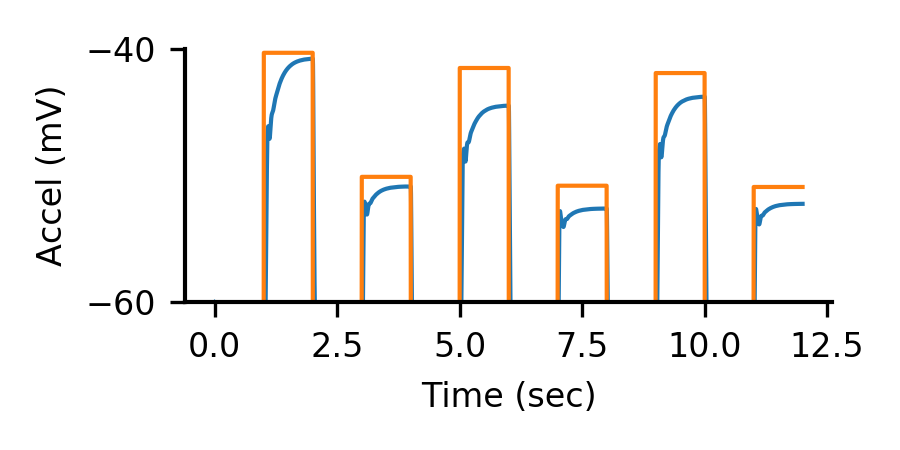
\includegraphics[width=3in]{results/TestAccelNeg}
}{%
\caption{Negative Acceleration Testing}
\label{fig:TestAccelNeg}
}
\end{floatrow}
\end{figure*}

Within the neuron network, acceleration is calculated primarily from actuator
pressures. The output is plotted compared with expected output. See \myref{fig:TestAccelPos} and \myref{fig:TestAccelNeg}.

\bbss{Torque Optimization}

The torque optimization network was tested as a complete network. See \myref{fig:TestTorqueOptimization}.
% TODO(buckbaskin): Figure of neuron controller torque optimization test

% TODO(buckbaskin): fix test data. This is broken back at the animatlab
\begin{figure}
\centering
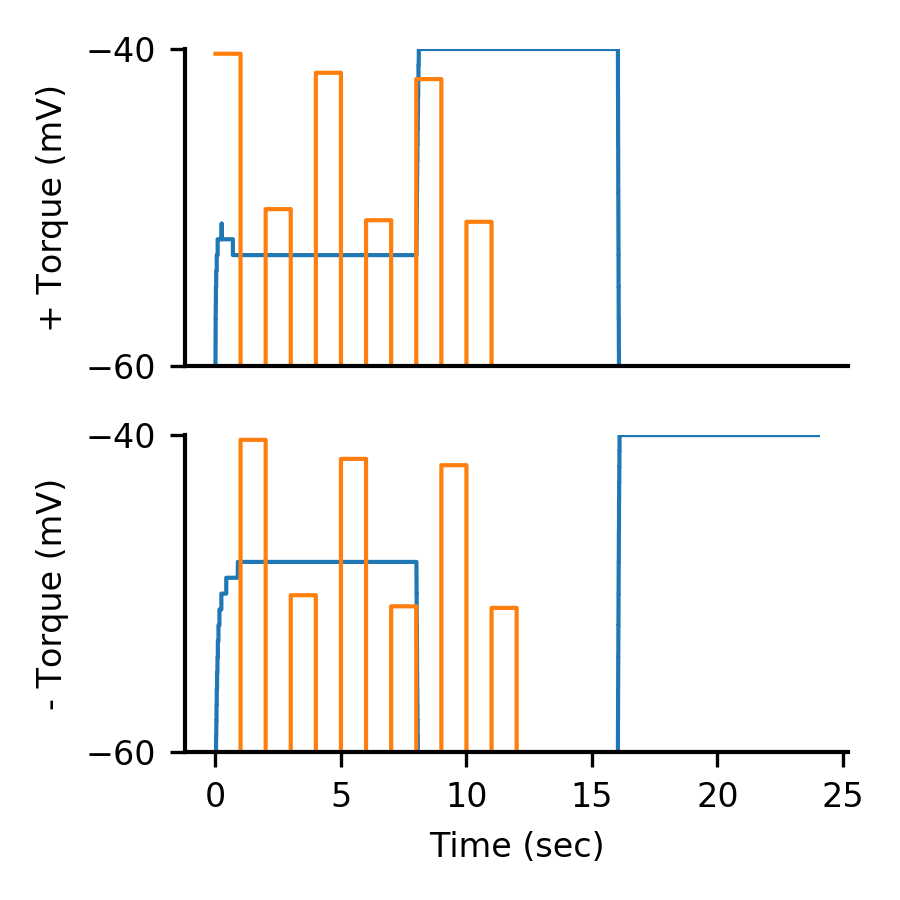
\includegraphics[width=3in]{results/TestTorqueOptimization}
\caption{Torque Optimization (Reference in orange)}
\label{fig:TestTorqueOptimization}
\end{figure}

The components for converting the torque to acceleration were also tested separately. See \myref{fig:TestT2A}.
% TODO(buckbaskin): Figure of neuron controller T2A
\begin{figure}
\centering
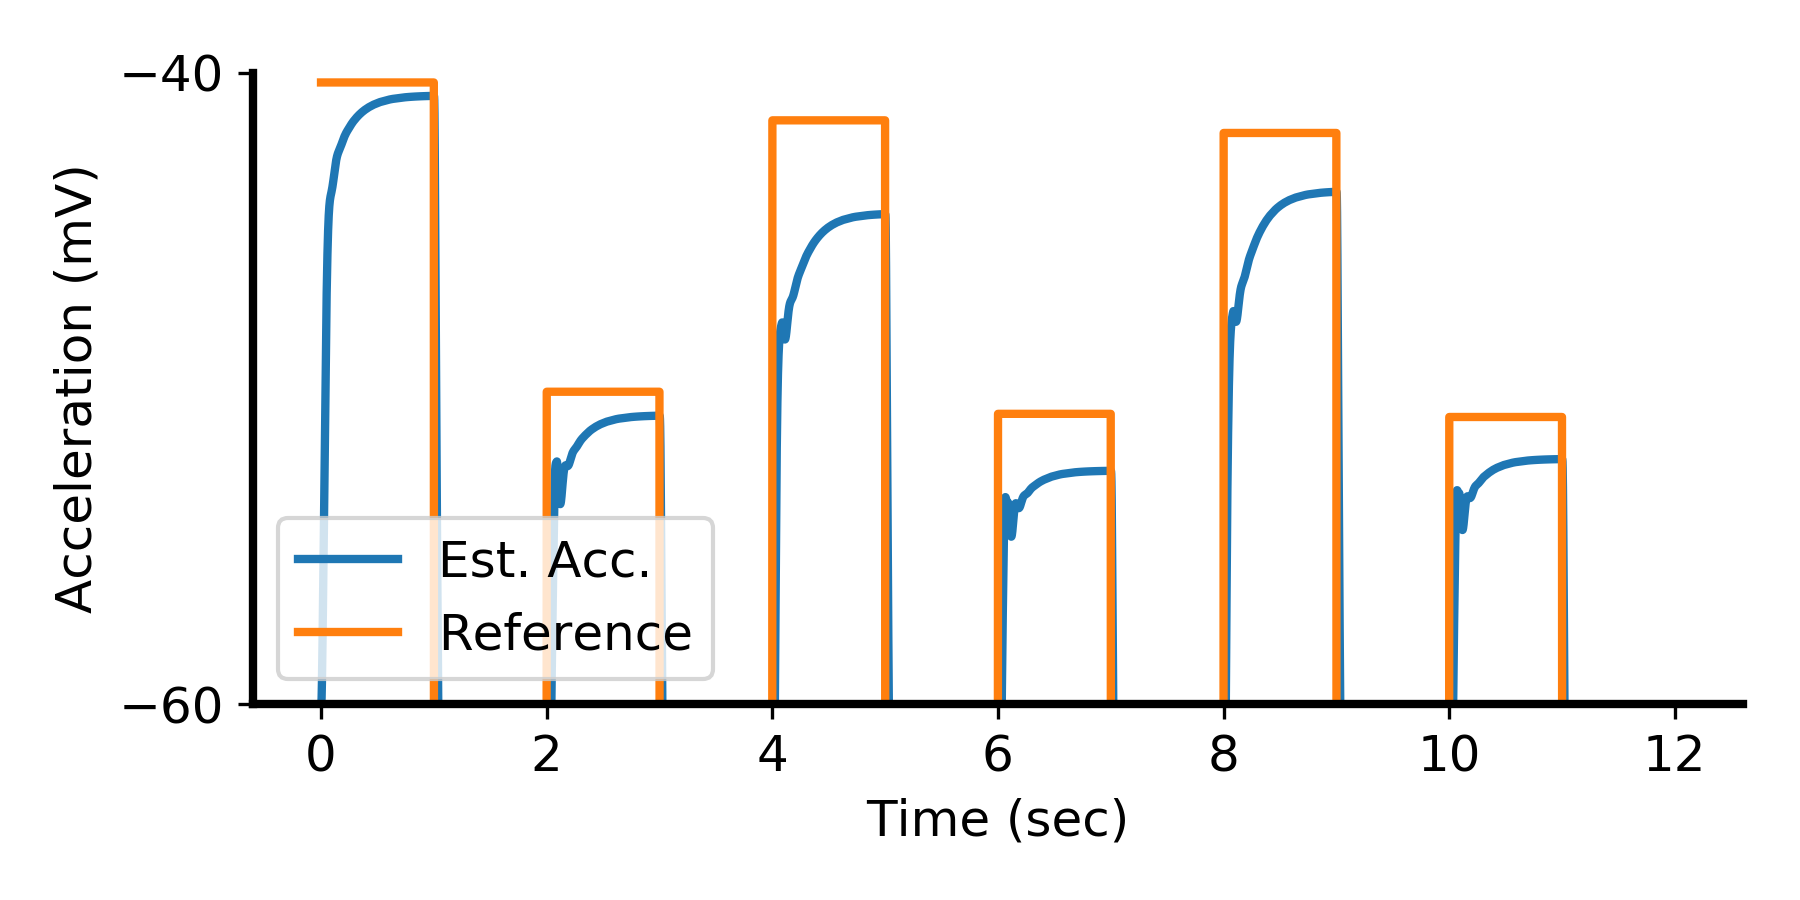
\includegraphics[width=3in]{results/TestAccelPos}
\caption{Converting applied torque to acceleration}
\label{fig:TestT2A}
\end{figure}

The components for converting the torque to pressure were also tested separately. See \myref{fig:TestT2P}.
% TODO(buckbaskin): Figure of neuron controller T2P
\begin{figure}
\centering
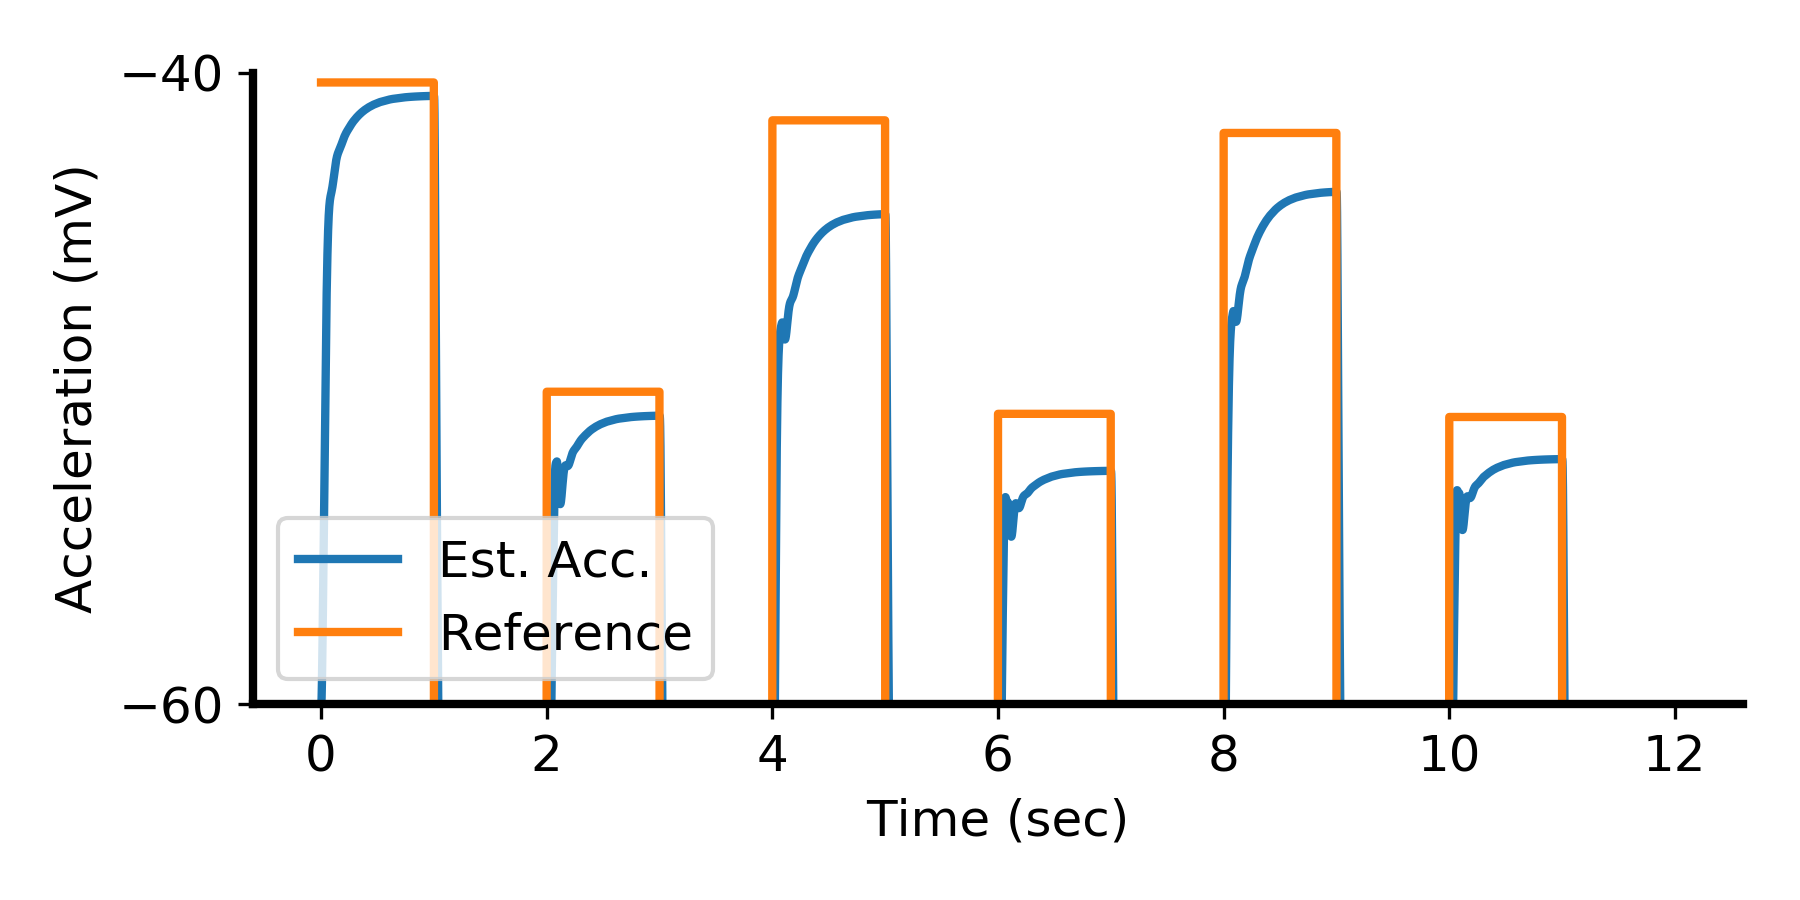
\includegraphics[width=3in]{results/TestAccelPos}
\caption{Converting desired torque to actuator pressure}
\label{fig:TestT2P}
\end{figure}

\bbss{System Modeling}

The system modeling network was tested as a complete network. See \myref{fig:SystemModel1}.
% TODO(buckbaskin): Figure of neuron controller system model tests (4x)
\begin{figure*}
\begin{floatrow}
\ffigbox{%
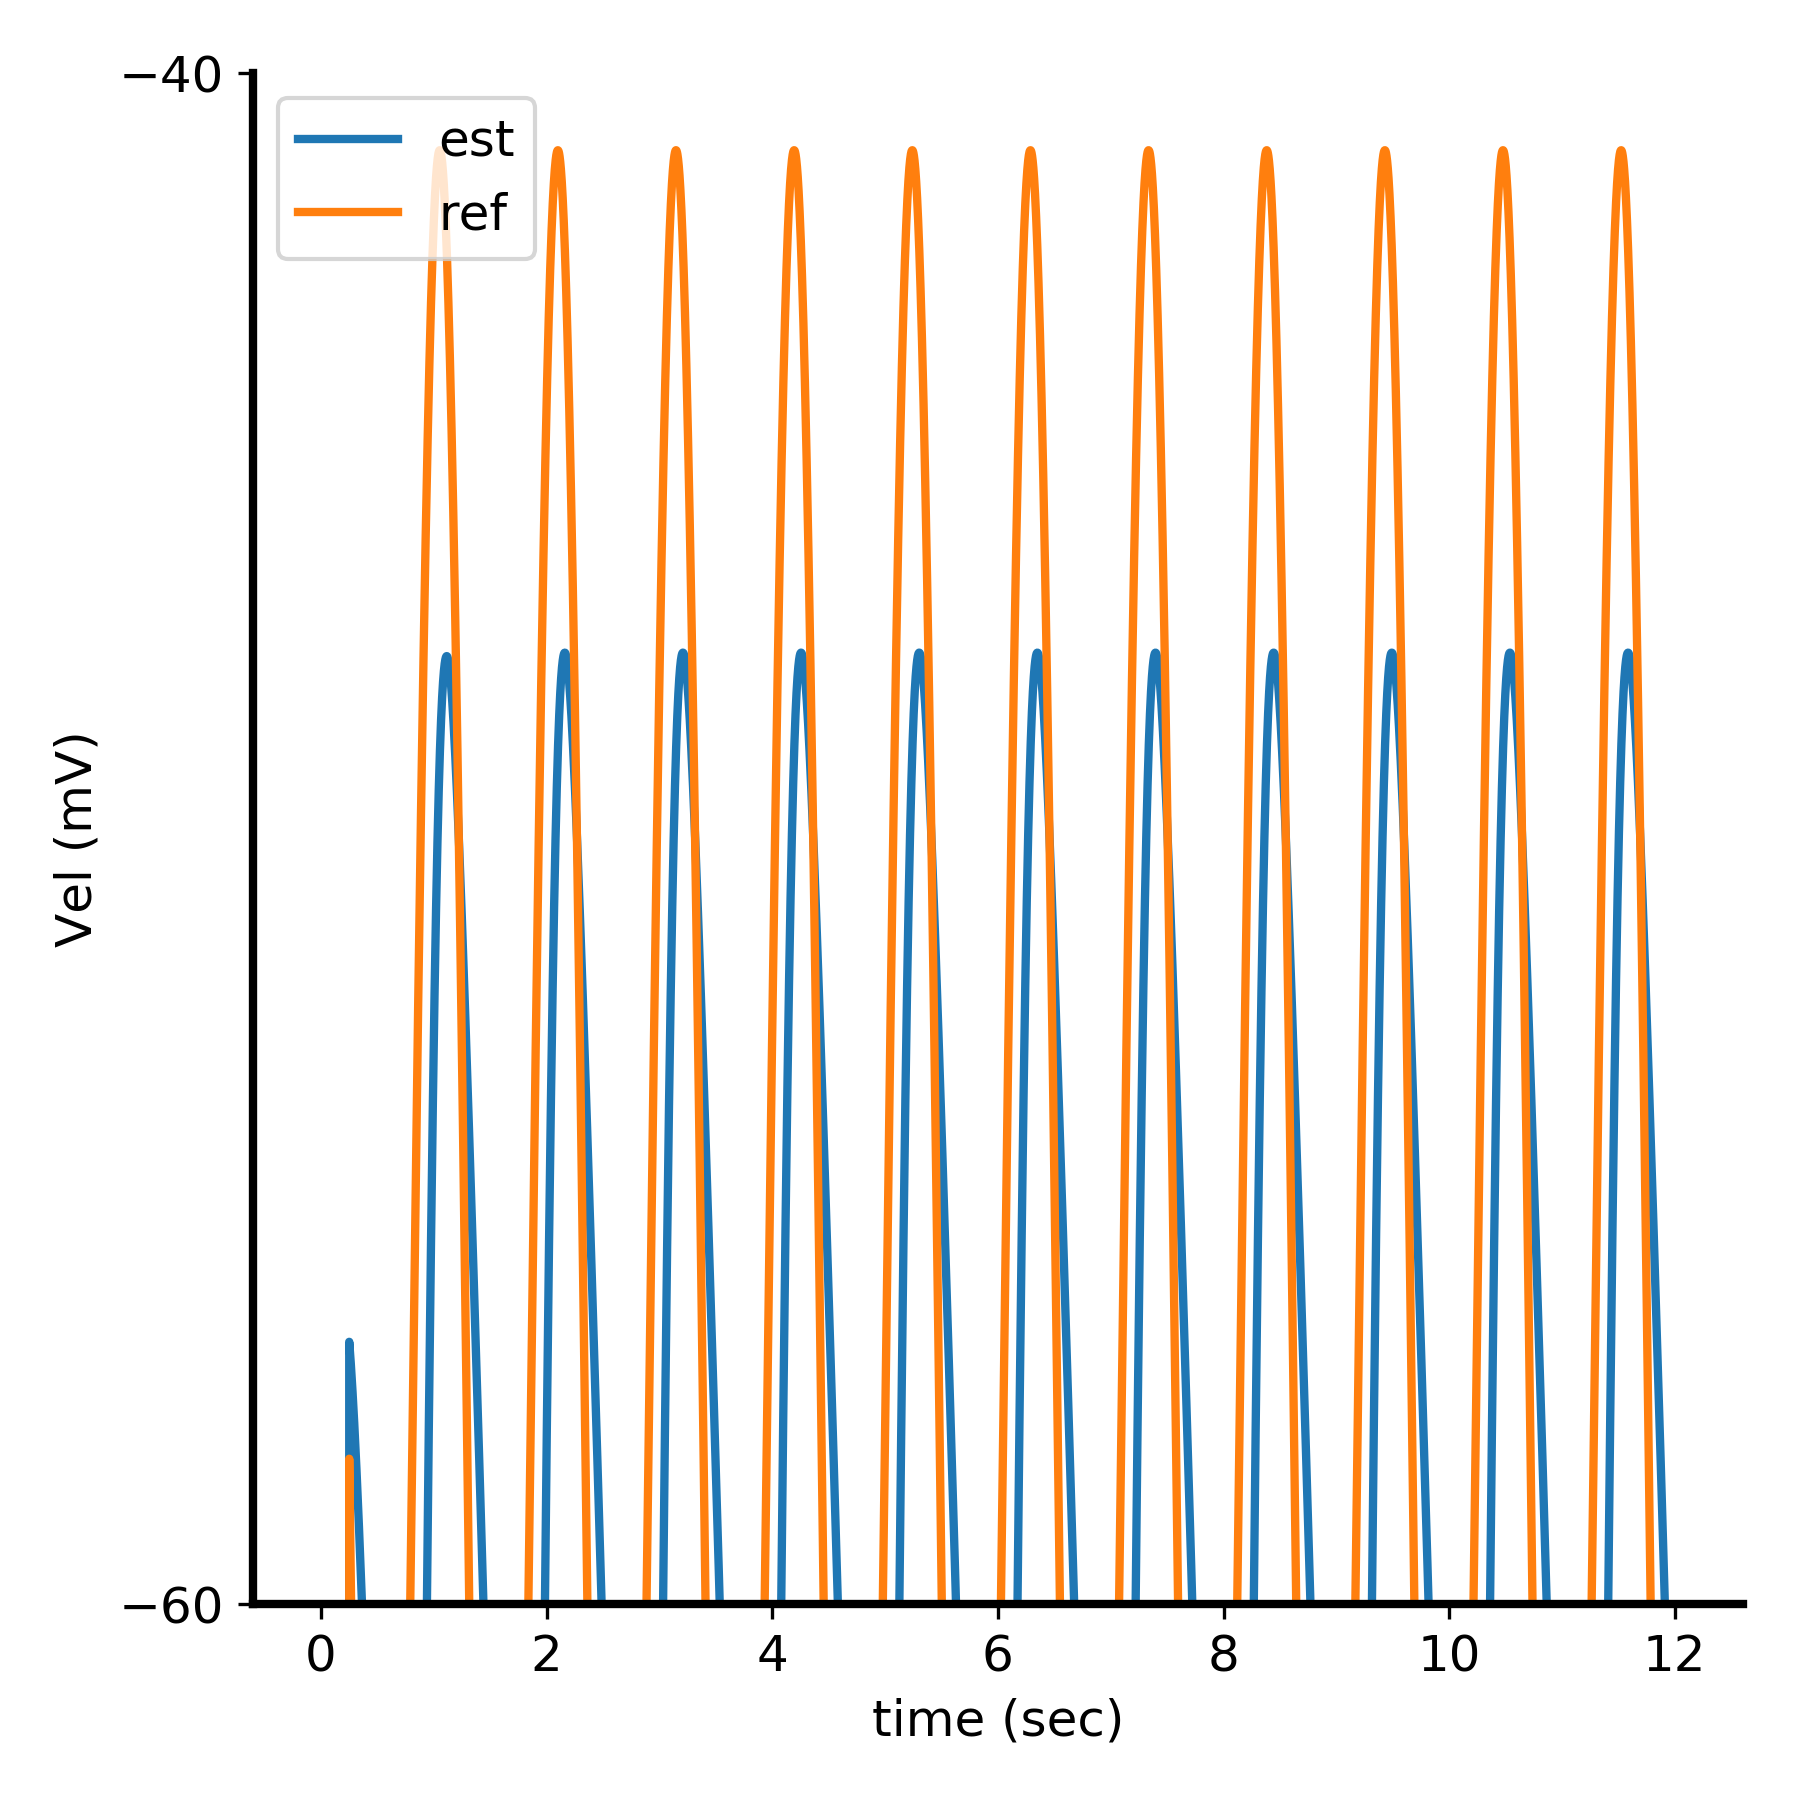
\includegraphics[width=3in]{results/TestVelPos}
}{%
\caption{System Model 1}
\label{fig:SystemModel1}
}

\ffigbox{%
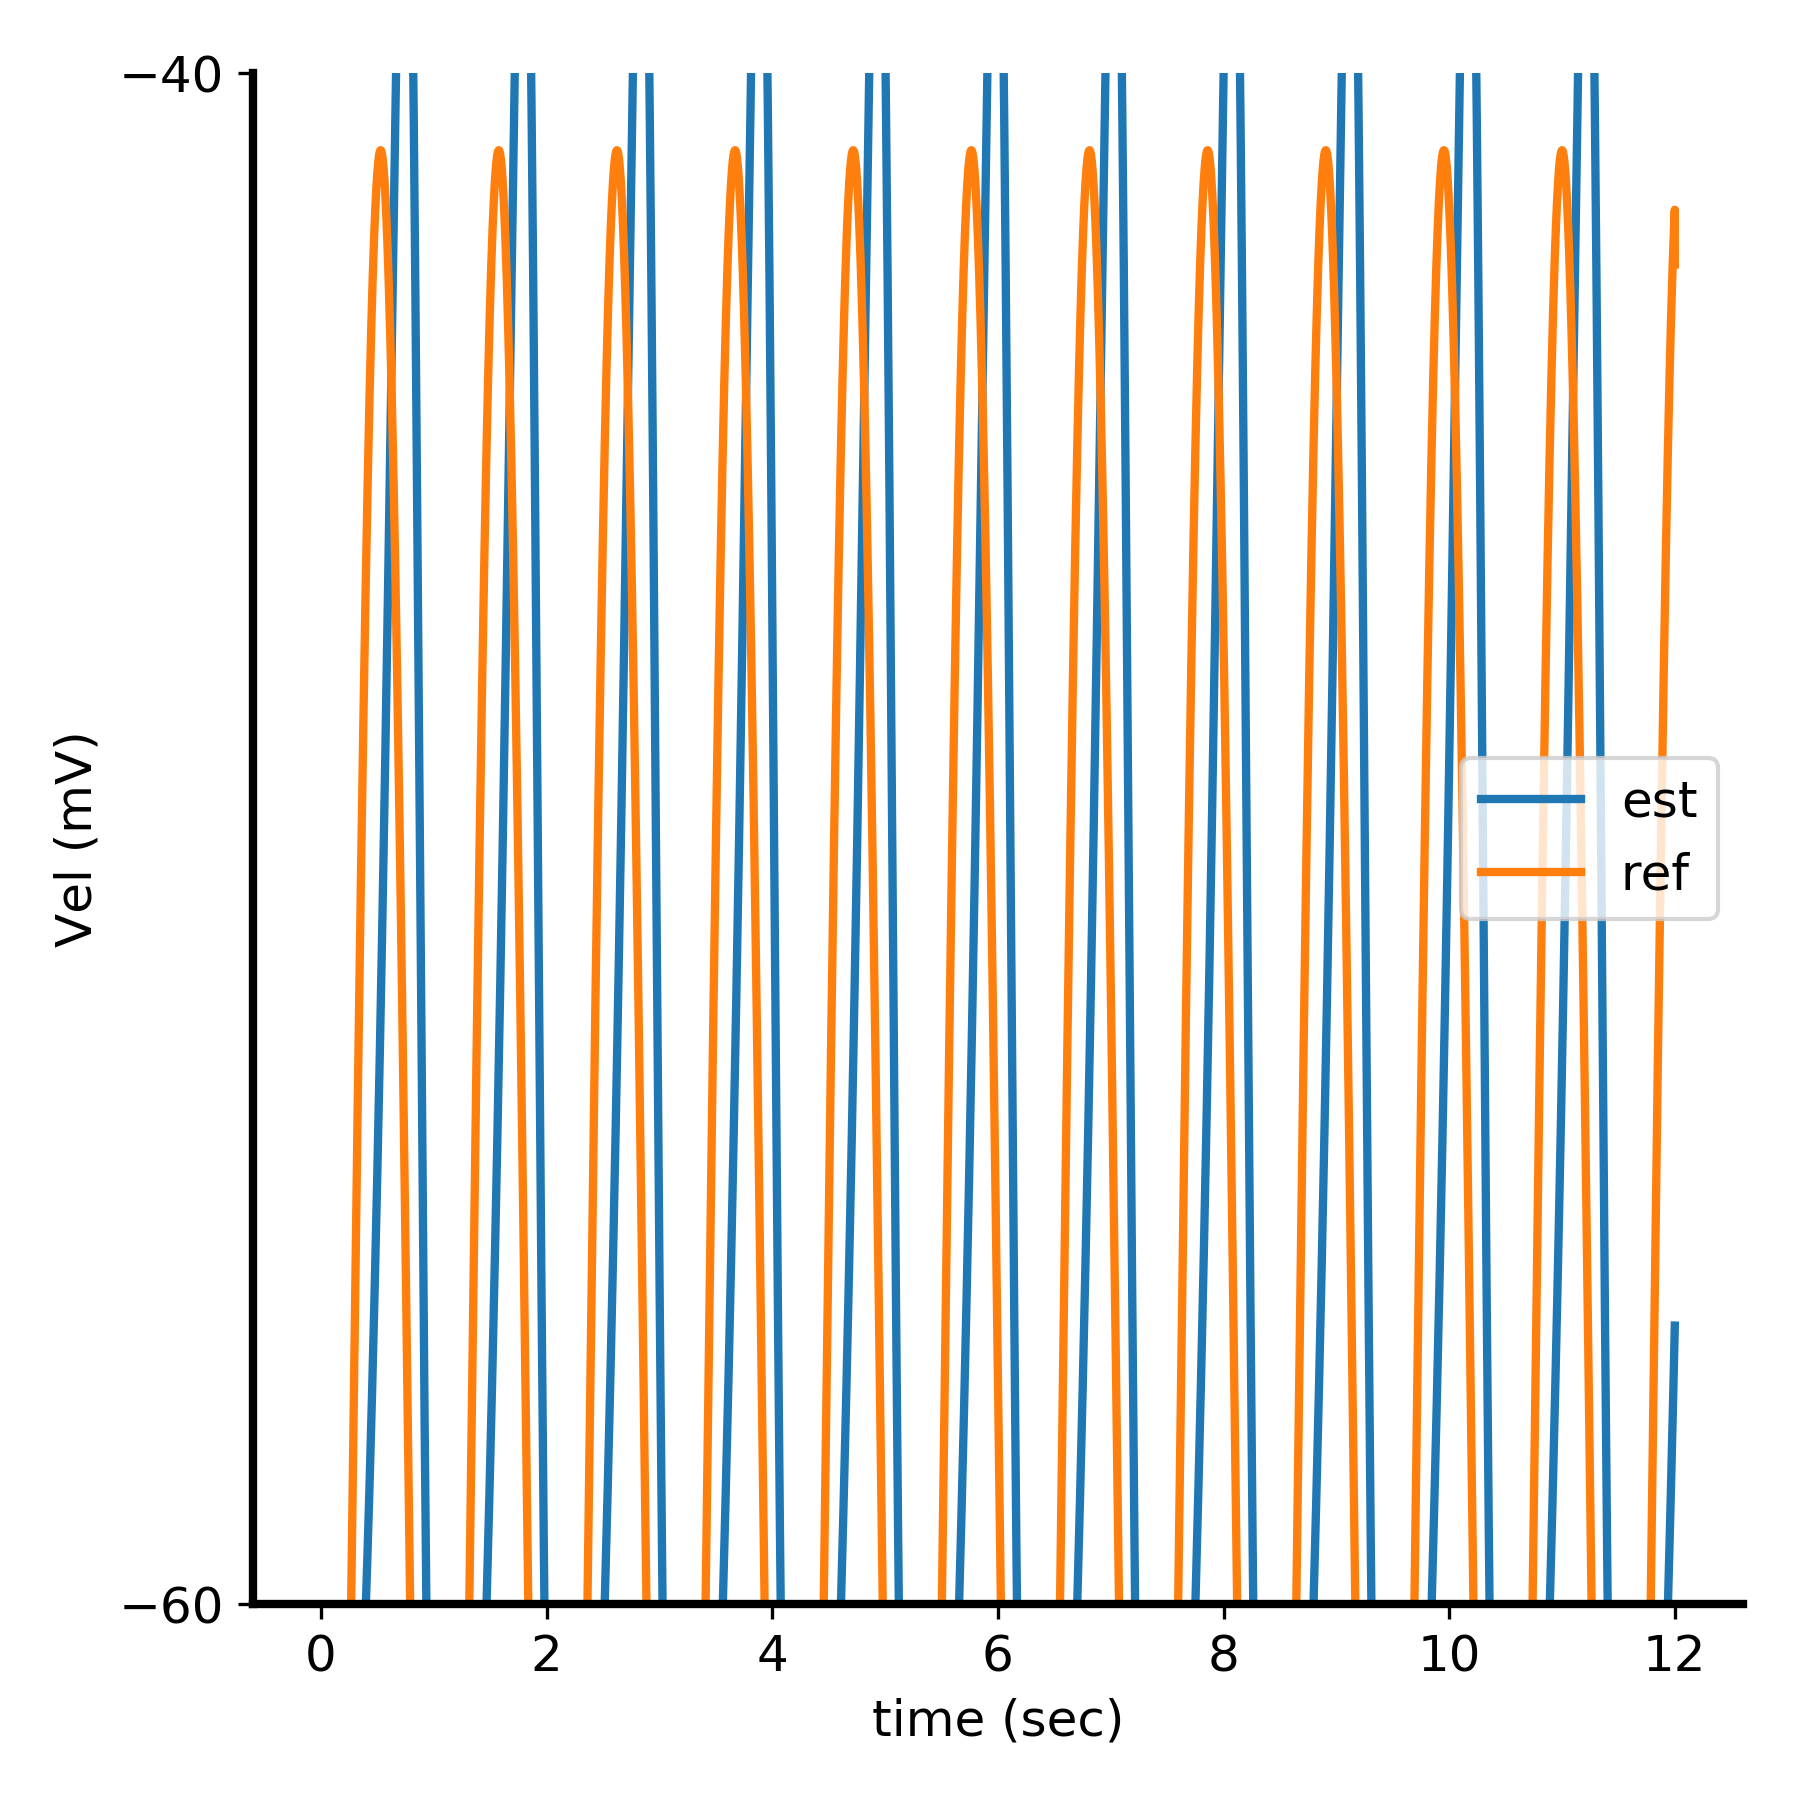
\includegraphics[width=3in]{results/TestVelNeg}
}{%
\caption{System Model 2}
\label{fig:SystemModel2}
}
\end{floatrow}
\begin{floatrow}
\ffigbox{%
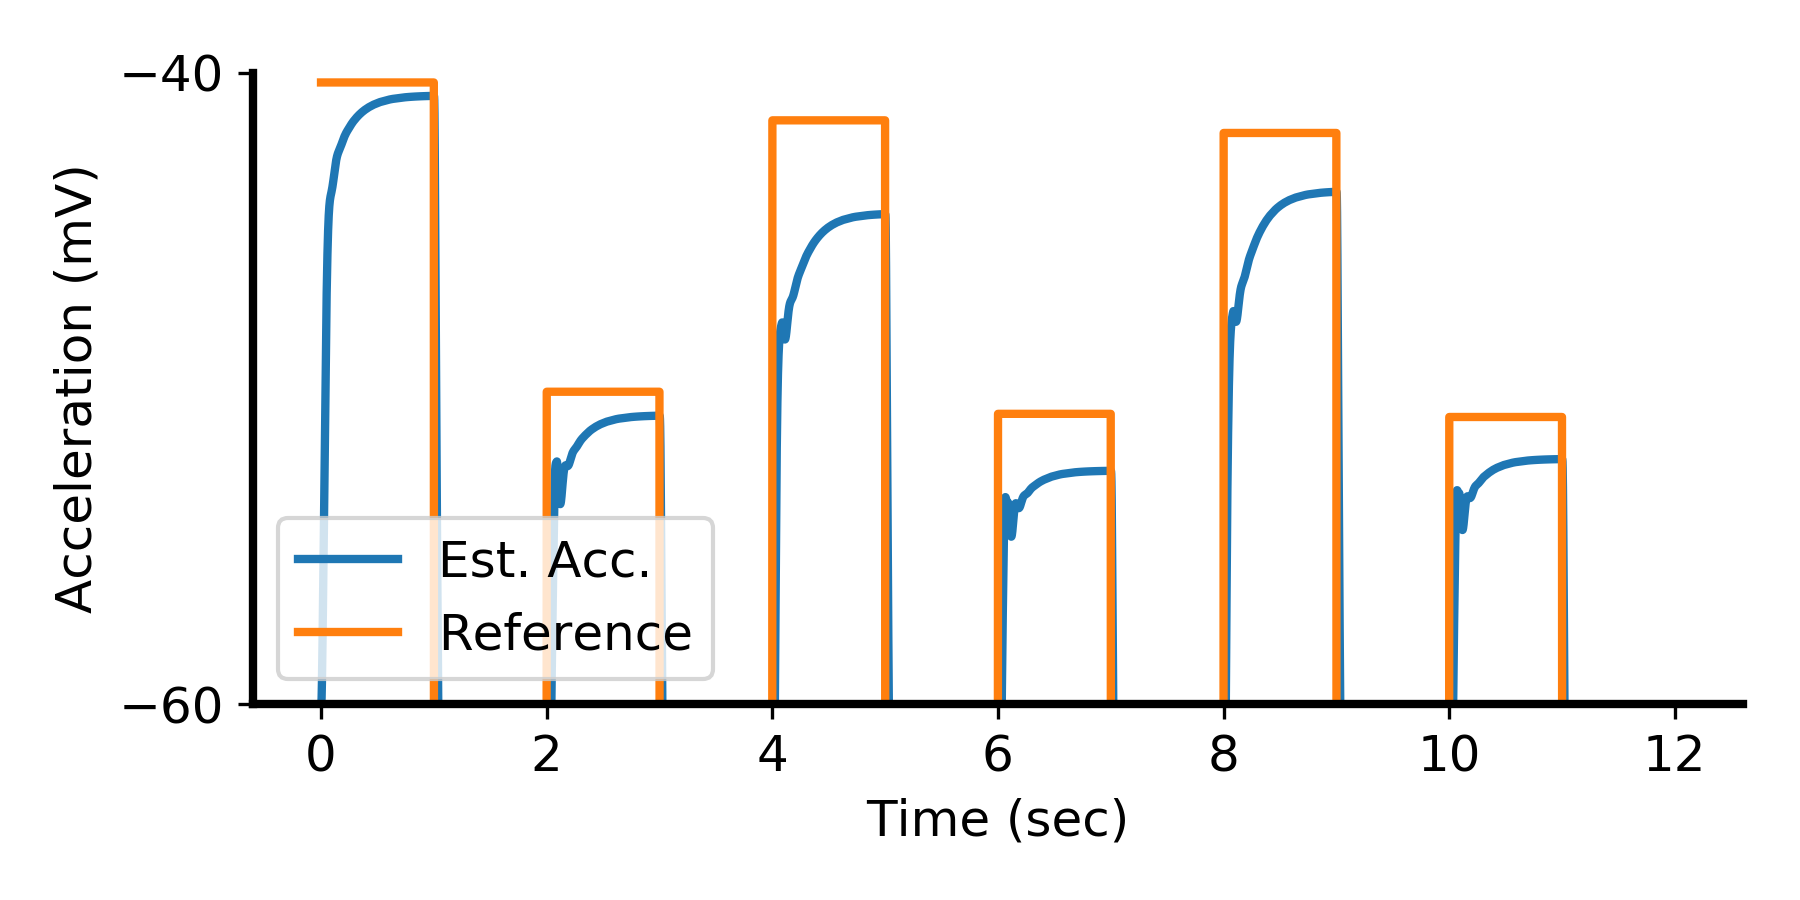
\includegraphics[width=3in]{results/TestAccelPos}
}{%
\caption{System Model 3}
\label{fig:SystemModel3}
}

\ffigbox{%
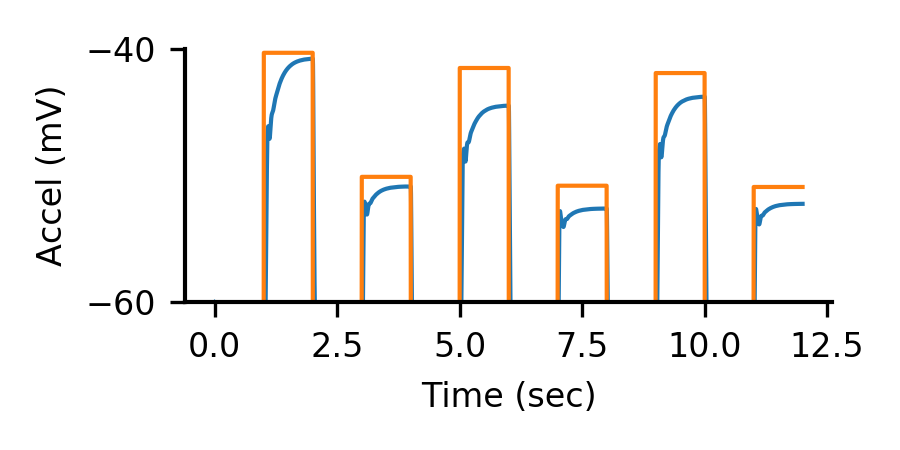
\includegraphics[width=3in]{results/TestAccelNeg}
}{%
\caption{System Model 4}
\label{fig:SystemModel4}
}
\end{floatrow}
\end{figure*}

\bbss{Overall}

% TODO(buckbaskin): Figure of neuron controller overall in step tests (fixed estimators)

\bbs{Discussion}
\label{chap:discussion}

Discuss accuracy of each piece

\bbs{Conclusion}
\label{chap:conclusion}

\newpage
\label{chap:references}
%TODO(buckbaskin): clean out extra unnecessary information from references.bib
\printbibliography[heading=bibintoc, title={Bibliography}]

\end{document}
